\documentclass[11pt,a4paper,fontset=none]{ctexart}
\usepackage[margin=1in]{geometry}
\usepackage{fontspec}
% Latin: Times New Roman (Mac / Windows) or TeX Gyre Termes (Linux); CJK: Songti / Heiti (Mac) or Fandol by file name
\IfFontExistsTF{Times New Roman}{\setmainfont{Times New Roman}}{\setmainfont{TeX Gyre Termes}}
\IfFontExistsTF{Songti SC}{%
  \setCJKmainfont{Songti SC}[BoldFont={Songti SC Bold}]%
  \setCJKsansfont{Heiti SC}\setCJKmonofont{Heiti SC}}{%
  \setCJKmainfont{FandolSong-Regular.otf}[BoldFont=FandolSong-Bold.otf]%
  \setCJKsansfont{FandolHei-Regular.otf}[BoldFont=FandolHei-Bold.otf]\setCJKmonofont{FandolHei-Regular.otf}}
\usepackage{amsmath,amssymb}
\usepackage{booktabs,array,multirow,makecell,tabularx}
\usepackage{graphicx,float,adjustbox}
\usepackage[table]{xcolor}
\usepackage[font=small,labelfont=bf,labelsep=quad]{caption}
\usepackage{enumitem}
\usepackage[numbers,square,sort&compress]{natbib}
\usepackage{xurl}
\usepackage[colorlinks=true,linkcolor=blue!50!black,citecolor=green!40!black,urlcolor=blue!60!black]{hyperref}
\setlist{nosep,leftmargin=1.6em}
\ctexset{section={format=\Large\bfseries\raggedright},subsection={format=\large\bfseries\raggedright},
         abstractname=摘要}
\setlength{\parskip}{0.25em}
\renewcommand{\arraystretch}{1.12}
\newcommand{\kimi}{Kimi K3.1 Pro}
\newcommand{\mini}{MiniMax M3.1 Flash}
\newcommand{\ds}{DeepSeek Flash V4.1-1017}
\newcommand{\lead}[1]{\textbf{#1}\quad}
\pagestyle{plain}

\title{\textbf{mmBench：多模态大模型评测基准}\\[0.3em]\large 技术报告}
\author{Albert Huang\\BAI AI Lab\\\small\url{https://github.com/BAI-AI-Lab/mmBench}}
\date{2026 年 10 月 31 日}

\begin{document}
\maketitle

\begin{abstract}
多模态大模型的评测通常把多种能力混在同一套题、同一个总分里：一道图表题可能同时考读字、读图和推理，一个总分也无法说明模型强在哪里、弱在哪里；而只报告单次运行的排名，又难以判断模型之间的差距是否真实。本文提出 mmBench，一个以能力画像为先、同时给出可量化排名的多模态评测基准。mmBench 把多模态能力划分为学科推理、视觉感知、图表、文档、空间、界面定位与视频时序 7 项，每项只考查一种技能、只使用一类答题形式，并在抽题时排除会考到其他能力的题；最终按固定随机种子从 11 个公开评测集中抽取 354 道题。所有题目用确定的规则评分，不使用模型裁判；每个模型每题作答 4 次，各项能力给出按题重抽样的 95\% 区间，两两比较采用按能力分层的配对 bootstrap。我们评测了 \kimi、\mini 与 \ds 三个模型：\kimi 以 85.3 分居首，领先另外两个模型约 11 分；后两者总分只差 0.7 分、统计上无法区分，能力画像却明显不同——\mini 在界面定位上高出 21.0 分，\ds 在空间上高出 11.5 分。我们把这些差异与厂商公开的技术要点逐条对照：\kimi 的坐标监督、\mini 的电脑操作方向与它们在界面定位上相对 \ds 的领先一致，\kimi 的空间推理声称相对 \mini 成立，\ds 在高分辨率界面上的短板与其接口的图片缩放上限相符，\mini 所称的生成速度则未能复现。按国内站标价，完成全部评测的费用分别约为 193 元、14 元与 28 元，三个模型每次调用的平均输出长度相差 5 倍。代码与题号清单已开源。
\end{abstract}

\section{引言}

多模态大模型已经能够回答学科问题、读懂图表与文档、在屏幕截图上操作界面，评测它们的基准也越来越多。然而，一个有用的评测不仅要回答“哪个模型更好”，还要回答“好在哪里”“差距是否可信”。我们认为现有的综合性评测在这三方面存在共同的问题：

\begin{itemize}[leftmargin=1.6em]
  \item \lead{能力相互混杂。}同一道题往往同时考查多种能力：学科题的图片可能是一张表格，图表题需要先读出图中的文字，界面题的目标可能是一段文字。分数低时，难以判断是哪一种能力不足；把这样的题合成一个总分，模型之间不同的能力结构也随之被抹平。
  \item \lead{评分引入额外噪声。}开放式答案常交给另一个模型判断对错，评分本身随裁判模型的版本与提示词变化，难以复现。
  \item \lead{排名缺少不确定性。}多数评测只报告单次运行的点估计，几分之差也被排成先后；而在几百道题的规模上，这样的差距常常在抽样误差之内。
\end{itemize}

针对这些问题，我们构建了 mmBench（图~\ref{fig:overview}）。它的核心思路是先定义互不重叠的能力，再从已有的公开评测集中挑选只考查该能力的题，并用统计方法明确区分“能分出高低的差距”与“分不出的差距”。本文的主要贡献如下：

\begin{itemize}[leftmargin=1.6em]
  \item 我们提出了一种能力正交的题库设计：7 项能力各对应一种技能和一类答题形式，并在抽题时逐题排除会考到其他能力的题，得到一个可复现的 354 题固定题库。
  \item 我们给出了同时支持能力画像与排名的评测协议：规则评分、每题 4 次采样、按题重抽样的区间、按能力分层的配对比较，以及“只有显著领先才分名次”的排名规则；并报告了这套题量所能分辨的最小差距。
  \item 我们用 mmBench 评测了三个国产多模态模型，分析了它们的能力画像、难度梯度、采样稳定性，以及以真实计费 token 计算的成本与效率；并给出一套把观测差异与厂商技术声称逐条对照的归因规则，区分可归因、不一致与无法检验的声称。
\end{itemize}

\begin{figure}[t]
  \centering
  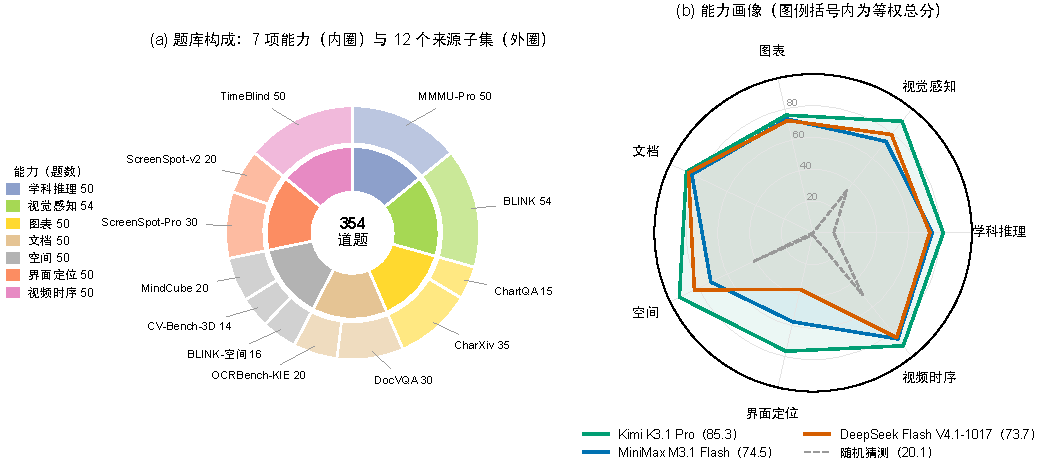
\includegraphics[width=\linewidth]{figures/fig1_overview.pdf}
  \caption{\textbf{mmBench 概览。}(a) 题库构成：内圈为 7 项能力及其题数，外圈为 12 个来源子集（BLINK 拆为感知与空间两部分）。(b) 三个模型的能力画像，虚线为随机猜测的期望得分。\kimi 在每一项上都处于最外圈；\mini 与 \ds 总分几乎相同，但在界面定位和空间两项上方向相反。}
  \label{fig:overview}
\end{figure}

\section{相关工作}

\paragraph{综合性多模态评测。}MMBench~\cite{mmbench} 以选择题覆盖约 20 个能力维度；MMMU~\cite{mmmu} 收集了大学水平的多学科图文问题，MMMU-Pro~\cite{mmmupro} 进一步过滤掉只看文字就能回答的题、把选项扩充到 10 个，并加入把题目印在图片里的版本。MMStar~\cite{mmstar} 指出许多评测题不看图也能答对，并人工筛选出依赖视觉的题目，用规则而非模型匹配答案。针对评测之间的冗余，Zhang 等人~\cite{redundancy} 用大量模型的得分相关性分析了维度内部与评测之间的重复。mmBench 与这些工作的目标不同：我们不追求覆盖面，而是让每项能力只考一种技能，以便画像中的每一项都可以单独解读。

\paragraph{单项能力评测。}mmBench 的题目全部来自以下公开评测集。视觉感知方面，BLINK~\cite{blink} 把深度估计、对应点匹配等经典视觉任务改写为选择题；学科推理方面使用 MMMU-Pro~\cite{mmmupro}。图表方面，ChartQA~\cite{chartqa} 以宽松准确率（数值允许 5\% 误差）评测图表问答，CharXiv~\cite{charxiv} 收集了 arXiv 论文中的真实图表并区分描述题与推理题。文档方面，DocVQA~\cite{docvqa} 提出了扫描文档问答与 ANLS 指标（ANLS 最早见于场景文字问答~\cite{anls}），InfographicVQA~\cite{infovqa} 关注信息图，OCRBench~\cite{ocrbench} 汇集了文字识别、场景文字问答与关键信息抽取等任务，后者包括 FUNSD~\cite{funsd} 与 SROIE~\cite{sroie} 等表单和收据数据。空间方面，Cambrian-1~\cite{cambrian} 提出的 CV-Bench 包含深度与距离判断，MindCube~\cite{mindcube} 考查在有限视角下的空间心理建模。界面定位方面，ScreenSpot~\cite{seeclick} 与其修订版 ScreenSpot-v2~\cite{osatlas} 覆盖手机、网页与桌面界面，ScreenSpot-Pro~\cite{screenspotpro} 面向高分辨率的专业软件。视频方面，TVBench~\cite{tvbench} 指出许多视频问答只看单帧或只看文字就能回答，并构建了真正依赖时序的题目；TimeBlind~\cite{timeblind} 以只在时间顺序上不同的成对视频考查时序理解；MMVU~\cite{mmvu} 则侧重专业领域知识。ZeroBench~\cite{zerobench} 收集了当前模型几乎全部答错的视觉推理题。

\paragraph{统计方法。}我们用 bootstrap~\cite{efron1979} 估计各项得分与两两差值的区间，并以题目为重抽样单位。

\section{为什么要按能力过滤题目}
\label{sec:overlap}

直接把上述评测集拼在一起，并不能得到互不重叠的能力。我们逐个检查了候选来源，发现能力交叉主要有以下几类：

\begin{itemize}[leftmargin=1.6em]
  \item \lead{学科题里的表格、统计图与截图。}MMMU-Pro 标准版共 1730 题，按其图片类型标注，含表格的有 359 题、含统计图的有 149 题、含截图的有 9 题（一题可以有多种类型）。这些题考的主要是读表、读图与读界面，与“学科推理”应考查的能力不同。
  \item \lead{感知评测中的空间与抽象推理子任务。}BLINK 的 14 个子任务中，相对深度、空间关系、多视角推理与目标定位考查的是空间关系；IQ 测试是抽象推理。
  \item \lead{文档评测中的图表与照片。}DocVQA 的部分问题针对页面上的插图或照片；OCRBench 的 1000 题中，有 200 道“文档问答”直接取自 DocVQA、ChartQA 与 InfographicVQA；InfographicVQA 本身是图表与文字的混合。
  \item \lead{界面定位中的文字目标与空间指点题。}点击一段文字，本质上是“读字＋定位”，会与文档能力重叠；反过来，若空间题用坐标作答，又会与界面定位共享“输出坐标”这一能力。
  \item \lead{视频评测中的专业知识题。}依赖专业领域知识的视频题，考查的主要是学科知识而非时序理解。
\end{itemize}

这些发现直接决定了第~\ref{sec:bench} 节的过滤规则：凡是会考到其他能力的子集、题型或答题形式，一律不收。

\section{mmBench 基准}
\label{sec:bench}

\subsection{设计原则}

\begin{itemize}[leftmargin=1.6em]
  \item \lead{一项能力只考一种技能。}题目所需的主要技能必须属于该项能力；会考到其他能力的题在抽题时排除（表~\ref{tab:caps}）。
  \item \lead{一项能力只用一类答题形式。}选择、短答案、坐标等形式各自只出现在少数能力中，其中坐标只用于界面定位，避免“不会按格式作答”这一种失败同时拉低多项能力。
  \item \lead{所有模型答同一套题。}题库由固定随机种子决定并以题号清单发布；视频按同一规则抽帧，所有模型看到的帧完全相同。
  \item \lead{只用确定的规则评分。}不使用模型裁判，同一份回答在任何时候都得到同一个分数。
\end{itemize}

\begin{table}[t]
  \centering
  \caption{\textbf{7 项能力的定义、来源与排除规则。}括号内为题数与难度档。难度按来源对当前模型是否已经饱和划分；MMMU-Pro 使用其自带的难度标签逐题分档。}
  \label{tab:caps}
  \small
  \begin{tabularx}{\linewidth}{@{}l>{\raggedright\arraybackslash}X>{\raggedright\arraybackslash}p{1.6cm}>{\raggedright\arraybackslash}p{3.6cm}>{\raggedright\arraybackslash}X@{}}
    \toprule
    能力 & 考查内容 & 答题形式 & 来源（题数，难度） & 排除的题 \\
    \midrule
    学科推理 & 结合学科知识的看图推理 & 10 选 1 & MMMU-Pro 标准版（50，L1--L3） & 图片为表格、统计图或截图的题；题目印在图片里的版本 \\
    视觉感知 & 计数、对应点、相似度、反射率、伪造检测、拼图、画风 & 选择题 & BLINK 的 9 个子任务（54，L2） & 深度、方位、多视角、定位子任务（归入空间）；IQ 测试 \\
    图表 & 读取数值、比较与趋势 & 短答案 & ChartQA（15，L1）；CharXiv 推理题（35，L3） & — \\
    文档 & 表单、版面、表格、收据等密集文字 & 短答案 & DocVQA（30，L1）；OCRBench 关键信息抽取（20，L2） & 针对插图或照片的问题；信息图；OCRBench 的文档问答子集 \\
    空间 & 深度、距离、方位与多视角心理建模 & 选择题 & CV-Bench 3D（14，L1）；BLINK 空间子任务（16，L2）；MindCube（20，L3） & 以坐标作答的指点题 \\
    界面定位 & 在截图上找到要点击的图标 & 坐标 & ScreenSpot-v2（20，L1）；ScreenSpot-Pro（30，L3） & 文字目标 \\
    视频时序 & 单看一帧无法回答的时序问题 & 是非、二选一 & TimeBlind（50，L3） & 依赖专业知识的视频题 \\
    \bottomrule
  \end{tabularx}
\end{table}

\subsection{构建流程}

构建流程如图~\ref{fig:pipeline} 所示。我们通过 Hugging Face 的 datasets-server 按行读取各来源的元数据，按表~\ref{tab:caps} 的规则逐题过滤，再以固定种子（seed = 0）抽样：同一来源内按子任务或难度标签轮流抽取，使各子任务与各难度档的题数尽量均衡。只有被抽中的题才会下载图片或视频；单张超过 7\,MB 的图片转为 JPEG，以满足各家接口的请求大小上限。视频按时长等分为 16 段，取每段中点的一帧，作为一组按时间排列的图片提供给模型。构建完成后，题号清单固定为 \texttt{samples/mm.json}，此后所有模型都回答这同一套题。

\begin{figure}[t]
  \centering
  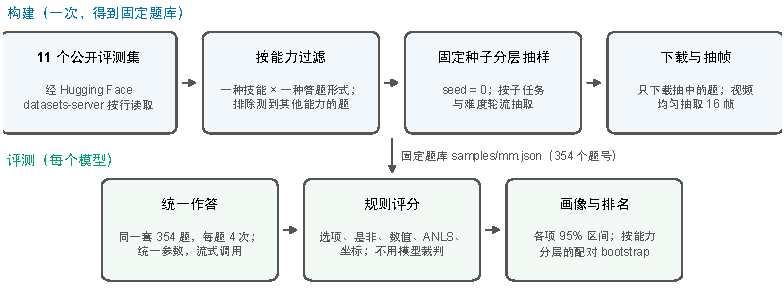
\includegraphics[width=\linewidth]{figures/fig2_pipeline.pdf}
  \caption{\textbf{构建与评测流程。}上行（实线框）只执行一次，得到固定题库；下行（虚线框）对每个模型执行，题目、抽帧与评分规则对所有模型完全相同。}
  \label{fig:pipeline}
\end{figure}

\subsection{统计信息}

表~\ref{tab:stats} 给出了各项能力的题数、题型、图片规模与随机猜测的期望得分。题型共 6 种：选择题 179 道、ANLS 短答案 50 道、坐标 50 道、文字短答案 37 道、是非题 25 道、数值短答案 13 道。文档与界面定位的图片分辨率最高（中位数分别为 3.10 与 3.69 百万像素），视频每题 16 帧。随机猜测的期望得分在各项之间差异很大，从图表和文档的 0 到视频时序的 50，等权平均为 20.1。

\begin{table}[t]
  \centering
  \caption{\textbf{各项能力的统计信息。}“随机猜测得分”为逐题计算的期望得分：选择题为选项数的倒数，是非题为 0.5，坐标题为目标框面积占整图的比例，短答案为 0。提示词词数包含作答格式说明。}
  \label{tab:stats}
  \small
  \begin{adjustbox}{max width=\linewidth}\begin{tabular}{lrlrrrr}
\toprule
能力 & 题数 & 题型（题数） & 每题图片数 & 分辨率中位数（MP） & 提示词词数 & 随机猜测得分 \\
\midrule
学科推理 & 50 & 选择 50 & 1.2 & 0.41 & 85 & 12.9 \\
视觉感知 & 54 & 选择 54 & 2.3 & 0.70 & 40 & 34.3 \\
图表 & 50 & 文字 37 / 数值 13 & 1.0 & 0.50 & 37 & 0.0 \\
文档 & 50 & ANLS 50 & 1.0 & 3.10 & 33 & 0.0 \\
空间 & 50 & 选择 50 & 2.1 & 0.31 & 61 & 42.0 \\
界面定位 & 50 & 坐标 50 & 1.0 & 3.69 & 53 & 1.3 \\
视频时序 & 50 & 是非 25 / 选择 25 & 16 帧 & 0.92 & 39 & 50.0 \\
\midrule
合计 & 354 & \multicolumn{4}{l}{难度：L1 96 题，L2 107 题，L3 151 题} & 20.1（等权） \\
\bottomrule
\end{tabular}
\end{adjustbox}
\end{table}

\section{评分与统计方法}
\label{sec:method}

\subsection{答案抽取与评分}

提示词要求模型在回答最后一行写出 “Answer: …”（附录~\ref{app:prompts}）。我们取回答中最后一个 “Answer:” 之后的内容作为最终答案，并按题型评分：

\begin{itemize}[leftmargin=1.6em]
  \item \lead{选择题与是非题：}与标准答案的选项字母或 yes/no 相同得 1 分；无法唯一确定字母时视为读不出答案。
  \item \lead{数值与文字短答案：}标准答案为数值时，取回答中的数值比较，允许带单位或 million、billion 等量级词；相对误差在 1\% 内得 1 分，ChartQA 按其宽松准确率放宽到 5\%。文字答案统一小写、去掉冠词与标点后要求完全相同。
  \item \lead{文档短答案：}采用 ANLS，即与最接近的标准答案的归一化编辑距离相似度，相似度低于 0.5 记 0。
  \item \lead{界面定位：}模型给出 0--1000 的相对坐标，换算到原图后落在目标框内得 1 分。
\end{itemize}

读不出答案、输出被截断或生成超时均记 0 分；接口在重试用尽后仍无回答的调用不计入，并在下次运行时重新请求。

\subsection{聚合与区间}

每个模型对每道题独立作答 $k=4$ 次，题目得分取 4 次的平均（avg@4）。某项能力的得分是该项各题得分的平均，换算为 0--100；总分是 7 项能力的等权平均，不按题数加权，以免题多的能力在总分中占更大比重。

各项得分的 95\% 区间来自 $B=2000$ 次按题重抽样：每次在每项能力内部有放回地抽取同样数量的题，重新计算各项得分与总分，取 2.5\% 与 97.5\% 分位数。两个模型的比较采用配对 bootstrap：每次重抽样对两个模型使用同一组题，得到分差的分布，从而消除题目难度带来的共同波动。

\subsection{排名规则}

模型的名次定义为 1 加上“明显强于它的模型数”，其中“明显强于”指两者总分差的 95\% 区间完全大于 0。两两总分差的区间包含 0 时，两个模型名次相同。我们另报告逐题比较的胜、平、负题数与精确符号检验。在本文的题量下，两两总分差的 95\% 区间半宽约为 $\pm 2.7$ 分，比这更小的差距无法区分。

\section{实验设置}
\label{sec:setup}

\subsection{被测模型}
\label{sec:models}

三个模型都是 2026 年 9--10 月发布的国产多模态模型，均可输入图像、默认开启思考。下面依次概述它们的能力、厂商公开的技术要点及其所针对的能力，以及官方评测成绩。以下内容均来自厂商的技术博客、技术报告、模型卡与接口文档（访问于 2026 年 10 月 30 日），分数为厂商自报，未经独立复现。

\paragraph{\kimi。}月之暗面于 2026 年 10 月 23 日发布，官方称它是 Kimi K3 的后训练版本，使用了大得多的后训练算力~\cite{kimik31}；K3 为 MoE 架构，总参数 2.8T、每 token 激活 104B，上下文 1M，可输入文本、图像与视频~\cite{kimik3}。K3.1 Pro 只公开了后训练层面的改进：在数百个领域上联合做强化学习，以大规模强化学习增强长程编程，并称它“擅长 3D 创作与空间推理”~\cite{kimik31}。架构与预训练继承自 K3，其中与本文能力直接相关的有四点~\cite{kimik3}：(1) 视觉编码器 MoonViT-V2（401M 参数）以下一 token 预测从头训练，经 2$\times$2 pixel-shuffle 压缩后可处理至 3584$\times$3584 像素的输入；(2) 训练时同时提供绝对坐标与归一化（[0,1]）坐标的监督，目的是实现“精确且与分辨率无关的定位”；(3) 在带 Python 沙箱的环境中做视觉推理的强化学习，模型可以裁剪、放大图片并做计算，面向 STEM 视觉推理、视觉谜题与图表理解；(4) 图像与视频共享全部参数，视频在帧内与帧间分解注意力，并沿时间维池化。K3 还在强化学习中给超出 token 预算的轨迹 $-1$ 的奖励，以提高思考的 token 效率。思考不能关闭，深度可选 low、high、max，默认 max~\cite{kimiquick}。官方成绩（max 深度，多模态评测取 4 次平均）：MMMU-Pro 84.1、CharXiv 推理题 89.0、OSWorld V2.1 79.6~\cite{kimik31}。

\paragraph{\mini。}MiniMax 于 2026 年 10 月 19 日上线接口、10 月 23 日开放权重；MoE 架构，总参数约 428B、每 token 激活约 23B，上下文 1M，可输入文本、图像与视频~\cite{minimaxm31}。厂商称 M3.1 Flash 沿用 M3 的核心架构，只做了三处改动：原先的前三层全注意力也改为稀疏注意力，路由专家与注意力路径做量化感知训练，并以 DSpark 投机解码代替原先的多 token 预测。这三处都面向推理速度与成本：官方称输出速度可达每秒 200 token 以上、中位数稳定在 170 以上，在线推理快近 3 倍、使用成本降低 70\%，并称在智能体、编程、电脑操作（Computer Use）与网络安全上带来“代际提升”~\cite{minimaxm31}。多模态能力来自前代 M3：从训练第 0 步起混合多种模态（原生多模态），并“能够操作桌面电脑”~\cite{minimaxm3}；厂商没有公开视觉编码器、界面定位或视频方面的训练方法。官方成绩：CharXiv 推理题 82.5（以 GPT-5.5 为裁判）、OSWorld 2.0 61.7、带工具的 BabyVision 91.0~\cite{minimaxm31}；前代 M3 的 MMMU-Pro 为 78.1、Video-MME（带字幕）为 85.4~\cite{minimaxm3}。

\paragraph{\ds。}DeepSeek 于 2026 年 9 月 10 日发布 V4.1-Flash，10 月 17 日更新为 1017 版，接口名与价格不变~\cite{ds1017}；多模态 MoE，主干 552B 参数、每 token 激活 8B（prefill）/ 16B（decode），另有 196B 的 Engram 条件记忆，上下文 1M，可输入图像，官方没有说明视频输入。技术报告~\cite{dsv41} 的主要创新是注意力与 KV cache 的压缩，面向长上下文与服务成本；报告明确说后训练“没有算法上的创新”，改动都在数据上。视觉方面：编码器 DeepSeek-ViT 从头训练，经 3$\times$3 pixel-unshuffle 把视觉 token 压缩为九分之一，支持至约 1344$\times$1344 像素；多模态数据从语言模型预训练开始即混入，其中包括面向“视觉定位与指点（grounding and pointing）”和 OCR 的领域数据，以及电脑操作轨迹。接口会把总像素超过约 1300$\times$1300 的图片等比缩小，每张图至多 1024 个 token~\cite{dsapi}。报告称它在视觉推理与专业图表理解的评测上超过 Kimi K3；1017 版称缩短了任务耗时与输出长度，并以自反馈强化学习改进端到端的项目开发~\cite{ds1017}。接口默认思考深度为 high，官方评测使用最高深度~\cite{dsapi,ds1017}。官方的多模态成绩只有两类：基座模型的 MMMU-Pro 56.5、CVBench 77.9、DocVQA 95.6（均为 4-shot），以及带工具的智能体评测，如 1017 版的 Chartography 83.0、BabyVision 92.5~\cite{ds1017}。

\subsection{调用设置}

三个模型均通过各自厂商的国内站、以兼容 OpenAI 的接口流式调用（表~\ref{tab:models}）。所有模型都不发送 temperature，使用厂商默认值；思考深度统一设为最高档：\mini 不能关闭思考、默认即最高档，\ds 的接口默认为 high，我们显式设为 max，与其官方评测一致。\kimi 与 \ds 的输出上限设为 96,000 token，远高于实际所需，\mini 不设上限。图片以 base64 内嵌，置于题目文字之前；视频题在 16 帧之前加一句“下面 N 张图片是从一段视频中按时间顺序均匀抽取的帧”，因此本文不经过各模型原生的视频输入通路。全部评测于 2026 年 10 月 31 日完成，每个模型 1416 次调用（354 题 × 4 次）。

\begin{table}[t]
  \centering
  \caption{\textbf{被测模型与调用设置。}单价为各厂商国内站的公开标价（元 / 百万 token），依次为输入（缓存未命中）、缓存命中与输出。\ds 在工作日 9:00--12:00 与 14:00--18:00（北京时间）为高峰价，其余时段为表中的空闲价，高峰价为空闲价的 2 倍。}
  \label{tab:models}
  \small
  \begin{adjustbox}{max width=\linewidth}
  \begin{tabular}{llccc}
    \toprule
    模型 & API 名称 & 思考深度 & 输出上限 & 单价（输入 / 缓存命中 / 输出） \\
    \midrule
    \kimi & \texttt{kimi-k3.1-pro} & max & 96,000 & 13 / 1.30 / 68 \\
    \mini & \texttt{MiniMax-M3.1-Flash} & 默认（max） & 不设 & 1 / 0.10 / 4 \\
    \ds & \texttt{deepseek-flash} & max（接口默认 high） & 96,000 & 1 / 0.02 / 4 \\
    \bottomrule
  \end{tabular}
  \end{adjustbox}
\end{table}

\subsection{归因规则}
\label{sec:attr-rule}

厂商声称的改进大多相对其上一代模型而言，而本文只评测了三个不同的模型，没有评测它们的前代，因此无法检验“是否比前代更好”。我们检验一个较弱的命题：在厂商声称改进的能力上，该模型相对另一个模型的位置，是否明显好于它们在总分上的相对位置。具体地，对模型 $A$、$B$ 与能力 $c$，令超出量为 $(s_A^c - s_B^c) - (s_A - s_B)$，即 $c$ 上的得分差减去等权总分差；它的 95\% 区间同样由配对 bootstrap 得到（每次重抽样同时重算两项）。一条声称记为\textbf{一致，可归因}，当且仅当：
\begin{itemize}[leftmargin=1.6em]
  \item 厂商指明了它针对的能力，且该能力能对应到 mmBench 的某一项能力；
  \item 该模型对另外两个模型中的至少一个，在这一项上的超出量区间完全大于 0。
\end{itemize}
对所有对比模型的超出量区间都包含 0 时，记为\textbf{未见相对优势}；超出量区间完全小于 0 时，记为\textbf{不一致}。对应不到 mmBench 的声称（如智能体编程、长上下文）记为\textbf{本文未测}；只是相对前代的数量声称（如“输出缩短”），本文没有前代对照，记为\textbf{无法检验}；可以直接测量的绝对数值（如生成速度）按测量值是否与声称相符判定。对于没有对应声称、但超出量显著的能力，我们也列出并记为\textbf{无对应声称}，不作归因。需要注意两点：其一，三个模型在某一项上得分都很接近时（例如接近天花板），总分落后的模型在这一项上的超出量自然为正，这种“一致”证据较弱；其二，这种归因只说明观测与声称不矛盾，而不是因果，三个模型在数据、规模与训练方法上同时不同，本文没有消融实验。

\section{实验结果}

\subsection{主要结果}

表~\ref{tab:main} 与图~\ref{fig:scores} 给出了三个模型在 7 项能力上的得分与 95\% 区间。

\begin{table}[t]
  \centering
  \caption{\textbf{主要结果（得分 0--100，越高越好 $\uparrow$）。}每列最高分加粗，次高分加下划线；灰色为按题重抽样的 95\% 区间。总分为 7 项能力的等权平均。}
  \label{tab:main}
  \small
  \setlength{\tabcolsep}{4.2pt}
  \begin{adjustbox}{max width=\linewidth}\begin{tabular}{l*{7}{c}c}
\toprule
模型 & 学科推理 & 视觉感知 & 图表 & 文档 & 空间 & 界面定位 & 视频时序 & \textbf{总分} \\
\midrule
随机猜测 & 12.9 & 34.3 & 0.0 & 0.0 & 42.0 & 1.3 & 50.0 & 20.1 \\
\midrule
Kimi K3.1 Pro & \textbf{82.0} & \textbf{89.8} & \textbf{76.0} & \textbf{88.6} & \textbf{93.5} & \textbf{76.5} & \textbf{91.0} & \textbf{85.3} \\
\multicolumn{1}{r}{\scriptsize\color{gray}95\% 区间} & {\scriptsize\color{gray}72.0--90.5} & {\scriptsize\color{gray}81.9--96.3} & {\scriptsize\color{gray}64.0--87.5} & {\scriptsize\color{gray}80.1--95.4} & {\scriptsize\color{gray}87.5--98.5} & {\scriptsize\color{gray}65.0--87.0} & {\scriptsize\color{gray}83.0--98.0} & {\scriptsize\color{gray}81.9--88.6} \\[2pt]
MiniMax M3.1 Flash & \underline{75.0} & 73.6 & \underline{73.5} & 84.8 & 71.5 & \underline{57.5} & \underline{85.5} & \underline{74.5} \\
\multicolumn{1}{r}{\scriptsize\color{gray}95\% 区间} & {\scriptsize\color{gray}64.0--85.0} & {\scriptsize\color{gray}63.9--82.4} & {\scriptsize\color{gray}62.0--85.0} & {\scriptsize\color{gray}75.0--92.7} & {\scriptsize\color{gray}60.5--81.5} & {\scriptsize\color{gray}47.0--68.0} & {\scriptsize\color{gray}76.5--93.0} & {\scriptsize\color{gray}70.6--78.2} \\[2pt]
DeepSeek Flash V4.1-1017 & 73.5 & \underline{79.2} & 72.5 & \underline{87.1} & \underline{83.0} & 36.5 & 84.5 & 73.7 \\
\multicolumn{1}{r}{\scriptsize\color{gray}95\% 区间} & {\scriptsize\color{gray}62.5--83.5} & {\scriptsize\color{gray}68.5--88.4} & {\scriptsize\color{gray}60.5--84.5} & {\scriptsize\color{gray}77.5--94.6} & {\scriptsize\color{gray}75.0--90.0} & {\scriptsize\color{gray}25.0--48.0} & {\scriptsize\color{gray}74.5--92.5} & {\scriptsize\color{gray}70.1--77.5} \\[2pt]
\bottomrule
\end{tabular}
\end{adjustbox}
\end{table}

\begin{figure}[t]
  \centering
  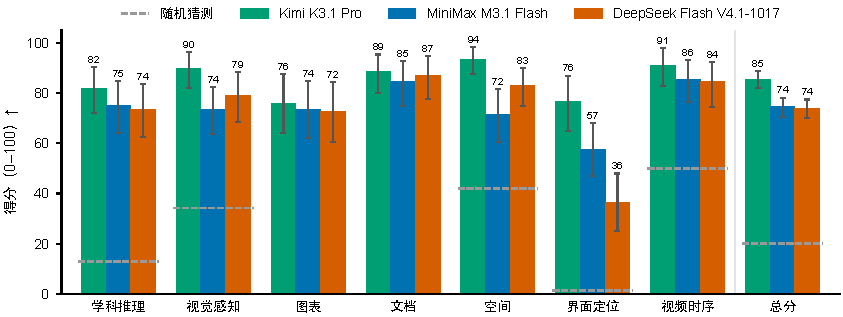
\includegraphics[width=\linewidth]{figures/fig3_scores.pdf}
  \caption{\textbf{各项能力得分与 95\% 区间。}虚线为随机猜测的期望得分。三个模型在每一项上都明显高于随机水平；图表与界面定位离满分最远。}
  \label{fig:scores}
\end{figure}

\lead{\kimi 在全部 7 项能力上得分最高，总分领先约 11 分。}它的总分为 85.3（81.9--88.6），比 \mini 高 10.9 分、比 \ds 高 11.6 分，两个差值的区间都完全大于 0；逐题比较，它分别有 90 道和 79 道题更好、15 道和 8 道题更差，符号检验 $p<0.001$。不过，它的领先并不在每一项上都显著：在图表上它与另外两个模型的差值区间都包含 0，在视频时序上与 \mini、在文档上与 \ds 的差值区间也包含 0（图~\ref{fig:pairwise}；逐项的逐题胜负见附录表~\ref{tab:wtl}）。

\lead{\mini 与 \ds 总分无法区分，能力画像却明显不同。}两者总分只差 0.7 分（区间 $-1.9$ 至 $+3.5$），逐题比较 55 道更好、52 道更差，符号检验 $p=0.85$，按排名规则并列第二。但在单项上，\mini 的界面定位高出 21.0 分（区间 13.5 至 29.0），\ds 的空间高出 11.5 分（2.5 至 21.5）、文档高出 2.3 分（0.6 至 4.3）。只看总分，这两个模型完全一样；看画像，它们适合的任务并不相同。这正是我们以能力画像为先的原因。

\lead{三个模型都远高于随机水平，图表与界面定位仍是共同的短板。}随机猜测的等权总分为 20.1，三个模型高出 53.6 至 65.2 分。图表一项三个模型都只有 72.5 至 76.0 分；界面定位的差距最大，从 36.5 到 76.5 分，其中高分辨率专业软件（ScreenSpot-Pro）的子集上 \ds 只有 8.3 分（附录表~\ref{tab:source}）。

\begin{figure}[t]
  \centering
  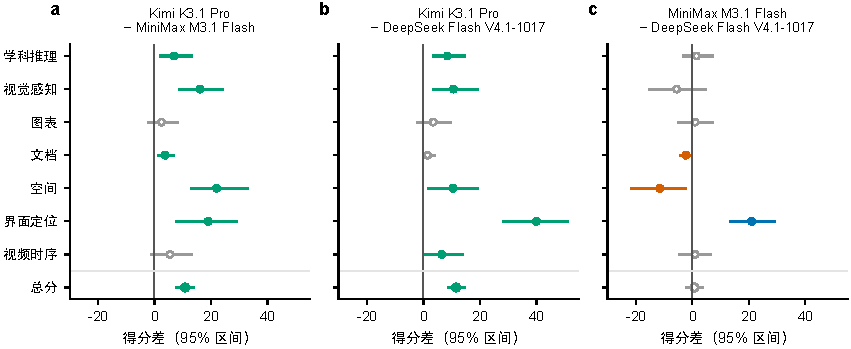
\includegraphics[width=\linewidth]{figures/fig4_pairwise.pdf}
  \caption{\textbf{逐项两两比较。}点为两个模型的得分差，横线为配对 bootstrap 的 95\% 区间。实心表示区间不含 0（差异显著），空心表示区间含 0；点的颜色为该项得分更高的模型。(c) 中两个模型的总分差不显著，但界面定位与空间两项方向相反且都显著。}
  \label{fig:pairwise}
\end{figure}

\subsection{观测到的差异能否归因于厂商声称的技术改进？}
\label{sec:attr}

表~\ref{tab:attr} 按第~\ref{sec:attr-rule} 节的规则，把第~\ref{sec:models} 节列出的每一条技术声称与本文的观测逐条对照。

\begin{table}[p]
  \centering
  \caption{\textbf{厂商声称与本文观测的对照。}“差”为该模型减去对比模型在该项上的得分差；“超出”为该项得分差减去两者的等权总分差，方括号内为配对 bootstrap 的 95\% 区间。判定规则见第~\ref{sec:attr-rule} 节；“一致”只表示观测与声称不矛盾，不表示因果。}
  \label{tab:attr}
  \scriptsize
  \renewcommand{\arraystretch}{1.1}\setlength{\tabcolsep}{4pt}
  \begin{tabularx}{\linewidth}{@{}>{\raggedright\arraybackslash}p{4.1cm}>{\raggedright\arraybackslash}p{1.4cm}>{\raggedright\arraybackslash}X>{\raggedright\arraybackslash}p{2.4cm}@{}}
\toprule
厂商声称（来源） & 对应能力 & 本文观测（得分差；超出总分差的部分及其 95\% 区间） & 判定 \\
\midrule
\multicolumn{4}{@{}l}{\textbf{Kimi K3.1 Pro}} \\
坐标监督（绝对与归一化坐标）；编码器支持至 3584$^2$ 像素（K3） & 界面定位 & 76.5，三者最高。相对 DeepSeek：差 40.0，超出 28.4 [18.2, 38.5]；相对 MiniMax：差 19.0，超出 8.1 [$-$1.4, 17.1]；ScreenSpot-Pro 60.8 & 一致，可归因（相对 DeepSeek） \\
“擅长 3D 创作与空间推理”（K3.1） & 空间 & 93.5。相对 MiniMax：差 22.0，超出 11.1 [3.0, 20.8]；相对 DeepSeek：差 10.5，超出 $-$1.1 [$-$8.8, 6.6] & 一致，可归因（相对 MiniMax） \\
带 Python 沙箱的视觉推理强化学习，面向 STEM 视觉推理与图表（K3） & 学科推理、图表 & 图表：相对 MiniMax：差 2.5，超出 $-$8.4 [$-$13.1, $-$3.2]；相对 DeepSeek：差 3.5，超出 $-$8.1 [$-$13.6, $-$2.3]。学科推理：超出 $-$3.9 [$-$9.1, 2.0]、$-$3.1 [$-$8.3, 2.5]。本文不提供工具 & 图表不一致；学科推理未见相对优势 \\
按 token 预算约束推理长度的强化学习（K3） & 思考效率 & 每次调用平均输出 932 token（中位数 221），三者最短 & 一致（token 计数跨厂商不可比） \\
视频通路（帧内、帧间分解注意力）；长程编程、金融、事实准确性 & 视频时序等 & 本文以帧图片输入视频，其余不在本文范围 & 本文未测 \\
\midrule
\multicolumn{4}{@{}l}{\textbf{MiniMax M3.1 Flash}} \\
电脑操作上的“代际提升”，OSWorld 2.0 61.7；M3 可操作桌面电脑 & 界面定位 & 57.5。相对 DeepSeek：差 21.0，超出 20.3 [13.3, 27.9]；相对 Kimi：差 $-$19.0，超出 $-$8.1 [$-$17.1, 1.4] & 一致，可归因（相对 DeepSeek） \\
全部层改为稀疏注意力、量化感知训练、DSpark 投机解码；称输出速度中位数 170 token/s 以上 & 生成速度 & 首个 token 之后的生成速度中位数 133 token/s，低于所称；DeepSeek 为 129 & 不一致（国内站、8 路并发、多图输入） \\
在线推理快近 3 倍、使用成本降低 70\%（相对前代） & — & 没有前代对照；全部评测费用 14.45 元，三者最低 & 无法检验 \\
从第 0 步起混合多种模态训练（M3） & 全部 & 没有指向具体能力 & 无法单独检验 \\
视频原生输入（M3 Video-MME 85.4）；智能体、编程、网络安全 & 视频时序等 & 本文以帧图片输入视频，其余不在本文范围 & 本文未测 \\
\midrule
\multicolumn{4}{@{}l}{\textbf{DeepSeek Flash V4.1-1017}} \\
“视觉定位与指点”领域数据、电脑操作轨迹 & 界面定位 & 36.5，三者最低。相对 Kimi：差 $-$40.0，超出 $-$28.4 [$-$38.5, $-$18.2]；相对 MiniMax：差 $-$21.0，超出 $-$20.3 [$-$27.9, $-$13.3]；ScreenSpot-v2 78.8、ScreenSpot-Pro 8.3 & 不一致 \\
接口把总像素超过约 1300$^2$ 的图片缩小，每图至多 1024 token（设计限制） & 高分辨率细节 & ScreenSpot-Pro 截图中位 5.8 MP，30/30 张被缩小，得分 8.3；DocVQA 26/30 张被缩小，仍得 94.3 & 与设计限制一致 \\
OCR 领域数据 & 文档 & 87.1。相对 Kimi：差 $-$1.5，超出 10.1 [6.6, 13.5]；相对 MiniMax：差 2.3，超出 3.0 [$-$0.1, 6.1]。DocVQA 三者 93.8--94.4，接近天花板 & 一致（相对 Kimi；该项接近天花板，证据弱） \\
视觉推理与专业图表的评测超过 Kimi K3 & 图表、学科推理 & 图表：相对 Kimi：差 $-$3.5，超出 8.1 [2.3, 13.6]。学科推理：超出 3.1 [$-$2.5, 8.3]、$-$0.8 [$-$5.9, 4.2] & 图表一致（相对 Kimi）；学科推理未见相对优势 \\
无空间方向的声称（只报告基座 CVBench 77.9） & 空间 & 83.0。相对 MiniMax：差 11.5，超出 12.2 [4.3, 21.4] & 无对应声称 \\
1017 版缩短输出长度（相对 0910 版） & — & 每次调用平均输出 4,685 token，三者最长；没有 0910 版对照 & 无法检验 \\
KV cache 压缩、Engram 条件记忆 & 长上下文、成本 & 本文单题输入短 & 本文未测 \\
\bottomrule
\end{tabularx}

\end{table}

\lead{界面定位上的差异与三家公开的做法相符。}\kimi 的训练同时监督绝对坐标与归一化坐标，\mini 把电脑操作列为主要改进方向；两者相对 \ds 在界面定位上的领先，分别比总分差多出 28.4 分（区间 18.2 至 38.5）与 20.3 分（13.3 至 27.9），可归因。\kimi 相对 \mini 的超出为 8.1 分，区间包含 0。\ds 的训练数据同样包含“视觉定位与指点”和电脑操作轨迹，界面定位却是三者最低；差距几乎全部来自高分辨率的 ScreenSpot-Pro（8.3 分，ScreenSpot-v2 为 78.8 分）。这与它公开的图片缩放上限相符：ScreenSpot-Pro 的截图中位数为 5.8 百万像素，30 张全部超过约 1300$\times$1300 的上限，被缩小后专业软件中本就很小的图标进一步缩小；同样有 26 张被缩小的 DocVQA，\ds 仍得 94.3 分，说明缩放对密集文字的影响远小于对小目标定位的影响。相比之下，\kimi 的编码器可处理至 3584$\times$3584 的输入。由于没有改变分辨率的对照实验，这一解释仍是推断。

\lead{空间、图表与文档的情况更复杂。}\kimi 的“空间推理”声称相对 \mini 成立（超出 11.1 分，区间 3.0 至 20.8），相对 \ds 则没有超出。\ds 在空间上相对 \mini 的超出同样显著（12.2 分），但厂商没有空间方向的声称，我们只作记录。图表一项三个模型的得分都很接近（72.5 至 76.0 分），因此总分领先的 \kimi 在这一项上的超出量显著为负，\ds 相对 \kimi 则显著为正：前者使 \kimi 带工具的视觉推理训练在本文的无工具条件下记为不一致，后者使 \ds 关于专业图表的声称记为一致，但两者其实反映的是同一个事实——图表这一项不能区分这三个模型。\ds 关于 OCR 数据的声称在文档上相对 \kimi 一致，但 DocVQA 上三者都在 93.8 至 94.4 分之间，接近天花板，证据较弱。学科推理上，\ds 与 \kimi 都没有显著的超出。

\lead{效率方面的声称多数无法检验，可检验的一条未能复现。}\mini 称输出速度中位数稳定在每秒 170 token 以上；本文测得它在首个 token 之后的生成速度中位数为每秒 133 token，与 \ds（129）相当。本文通过国内站调用、8 路并发并输入多张图片，这些条件都可能拉低速度。“快近 3 倍”“输出缩短”等相对前代的声称，本文没有前代对照，无法检验。\kimi 的平均输出最短（每次调用 932 token），与其按 token 预算约束推理长度的训练方法方向一致，但各家的分词方式不同，token 数只能粗略比较。

\subsection{与官方成绩的对照}
\label{sec:official}

表~\ref{tab:official} 列出了厂商在本文来源评测集上自报的成绩。本文只使用各评测集经过过滤的子集，评分也不同，两者不能直接比较，这里只看方向。MMMU-Pro 上本文的得分比厂商自报低 2.1 至 7.1 分；两边都是 \kimi 最高，\mini 与 \ds 的先后则相反，但厂商成绩中 \mini 一行是前代 M3 的成绩，\ds 一行由月之暗面测得。CharXiv 推理题上，本文的得分比厂商自报低 10.6 至 17.6 分，但先后同样一致（\kimi{} $>$ \mini{} $>$ \ds）。差距的主要原因是评分方式不同：厂商以模型为裁判，本文使用规则评分；本文还发现了少量规则误判（第~\ref{sec:robust} 节）。\ds 的 DocVQA 与 CV-Bench 只有基座模型的成绩，与本文评测的接口模型不同。

\begin{table}[!htbp]
  \centering
  \caption{\textbf{厂商自报成绩与本文对应子集的得分。}\ds 的 MMMU-Pro 与 CharXiv 成绩取自 \kimi 博客中的对比表（由月之暗面测得，max 深度）；\mini 的 MMMU-Pro 为前代 M3 的成绩。本文子集为 4 次平均。}
  \label{tab:official}
  \small
  \begin{adjustbox}{max width=\linewidth}\begin{tabular}{lllrl}
\toprule
评测 & 模型 & 厂商自报 & 本文子集 $\uparrow$ & 主要口径差异 \\
\midrule
\multirow{3}{*}{MMMU-Pro 标准版} & Kimi K3.1 Pro & 84.1 & 82.0 & \multirow{3}{*}{\parbox{4.2cm}{\raggedright 本文排除表格、统计图与截图题，50 题}} \\
 & MiniMax M3.1 Flash & 78.1（前代 M3） & 75.0 &  \\
 & DeepSeek Flash V4.1-1017 & 80.6（Kimi 博客中的对比值） & 73.5 &  \\
\midrule
\multirow{3}{*}{CharXiv 推理题} & Kimi K3.1 Pro & 89.0 & 71.4 & \multirow{3}{*}{\parbox{4.2cm}{\raggedright 本文 35 题、规则评分；厂商用模型裁判}} \\
 & MiniMax M3.1 Flash & 82.5（GPT-5.5 裁判） & 67.9 &  \\
 & DeepSeek Flash V4.1-1017 & 77.0（Kimi 博客中的对比值） & 66.4 &  \\
\midrule
\multirow{1}{*}{DocVQA} & DeepSeek Flash V4.1-1017 & 95.6（基座，4-shot，模型裁判） & 94.3 & \multirow{1}{*}{\parbox{4.2cm}{\raggedright 本文为接口模型、ANLS}} \\
\midrule
\multirow{1}{*}{CV-Bench} & DeepSeek Flash V4.1-1017 & 77.9（基座，4-shot，全集） & 98.2 & \multirow{1}{*}{\parbox{4.2cm}{\raggedright 本文只用 3D 子集，14 题}} \\
\bottomrule
\end{tabular}
\end{adjustbox}
\end{table}

\subsection{难度越高，模型之间的差距是否越大？}

图~\ref{fig:tiers}(a) 把所有能力合在一起，按难度档计算得分。在 L1 上三个模型相差不到 5 分（88.1 至 92.8），到 L3 时差距扩大到 18.2 分（61.3 至 79.5）。\kimi 从 L1 到 L3 只下降 13.3 分，\mini 与 \ds 分别下降 24.8 与 26.8 分。需要注意的是，难度档按来源划分，不同档位对应的能力构成并不相同（例如 L3 包含全部视频题与 ScreenSpot-Pro），这里的趋势混合了难度与能力两方面的因素。

\begin{figure}[t]
  \centering
  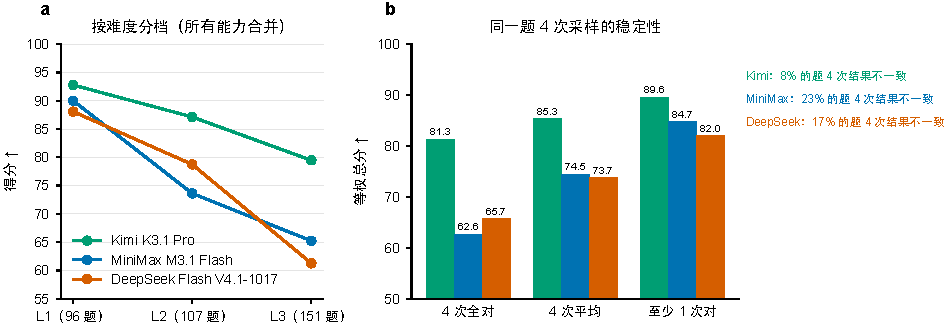
\includegraphics[width=\linewidth]{figures/fig6_tiers_sampling.pdf}
  \caption{\textbf{难度分档与采样稳定性。}(a) 按难度档的得分（所有能力合并）。(b) 同一题 4 次采样的三种聚合：4 次全对（all@4）、4 次平均（avg@4，即本文的主指标）与至少 1 次答对（pass@4）。\kimi 的三者最接近，4 次结果不一致的题只占 8\%。}
  \label{fig:tiers}
\end{figure}

\subsection{同一道题答 4 次，结果是否稳定？}

图~\ref{fig:tiers}(b) 比较了三种聚合方式。\kimi 只有 30 道题（8\%）的 4 次结果不一致，pass@4 比 avg@4 高 4.3 分；\mini 有 82 道题（23\%）不一致，pass@4 比 avg@4 高 10.2 分；\ds 为 61 道题（17\%）、高 8.3 分。也就是说，\mini 与 \ds 的不少错误并非“不会”，而是“不稳定”：多次采样再投票或挑选，有望带来比 \kimi 更大的提升。这也说明单次运行的评测会给这两个模型带来更大的随机误差，每题多次采样对于可靠排名是必要的。

\subsection{哪些题所有模型都答不对？}

以题目得分不低于 0.5 记为答对，354 道题中有 246 道（69\%）三个模型都答对，38 道（11\%）三个模型都答错。全错的题集中在图表（10 道）、界面定位（8 道）与学科推理（7 道），而空间（1 道）与视频时序（2 道）最少。界面定位也是三个模型分歧最大的一项：50 道题中只有 19 道三个模型都答对。

\section{成本与 token 效率}
\label{sec:cost}

\begin{table}[t]
  \centering
  \caption{\textbf{token 用量与费用（越低越好 $\downarrow$）。}token 数为各厂商接口返回的计费用量，不同厂商对同一张图片的计数方式不同，因此只有费用可以跨模型比较。费用按表~\ref{tab:models} 的国内站标价计算；\ds 的全部调用都在空闲时段（周六），按高峰价约为 55.02 元。美元为各厂商国际站标价，仅供参考。}
  \label{tab:cost}
  \small
  \begin{adjustbox}{max width=\linewidth}\begin{tabular}{lrrrrrrrr}
\toprule
 & \multicolumn{4}{c}{每次调用平均 token} & & \multicolumn{3}{c}{全部 1416 次调用的费用 $\downarrow$} \\
\cmidrule(lr){2-5}\cmidrule(lr){7-9}
模型 & 输入 & 其中缓存命中 & 输出（中位数） & 思考占输出 & 延迟中位数（秒）$\downarrow$ & 元 & 元 / 题 & 美元参考 \\
\midrule
Kimi K3.1 Pro & 5,973 & 425 & 932（221） & 97.8\% & 11.4 & 192.69 & 0.544 & \$29.03 \\
MiniMax M3.1 Flash & 5,407 & 2,876 & 1,847（250） & 99.3\% & 4.3 & 14.45 & 0.041 & \$2.17 \\
DeepSeek Flash V4.1-1017 & 2,257 & 1,601 & 4,685（709） & 99.5\% & 6.1 & 27.51 & 0.078 & \$4.13 \\
\bottomrule
\end{tabular}
\end{adjustbox}
\end{table}

表~\ref{tab:cost} 与图~\ref{fig:cost} 汇总了三个模型的 token 用量与费用。所有数字都来自接口返回的计费用量，而不是我们自己估算的 token 数。

\lead{\kimi 的领先以 7 到 13 倍的费用为代价。}按国内站标价，完成全部 1416 次调用，\kimi 约需 192.69 元，是 \ds（27.51 元）的 7.0 倍、\mini（14.45 元）的 13.3 倍；折合每题（4 次作答）分别为 0.544 元、0.078 元与 0.041 元。在本次评测的一段计费窗口中，\kimi 账户的实际扣费比按标价估算的高约 17\%，可能来自缓存写入等其他计费项，因此其实际费用可能更高。\mini 本次使用的是订阅套餐，表中为按量计费的等价费用。

\lead{输出更长并不意味着答得更好。}\ds 每次调用平均输出 4,685 个 token，是 \kimi（932 个）的 5 倍，总分却低 11.6 分。三个模型的输出中，思考内容都占 97\% 以上；输出长度的分布都有很长的尾巴，\ds 的中位数（709）只有均值的约 15\%，\kimi 的中位数更是只有 221。按能力看（图~\ref{fig:tokens}），\ds 在学科推理与空间上的平均输出分别达到 9.7k 与 7.8k token，而文档题三个模型都只需 144 至 200 个 token（各项的输入与输出 token 见附录表~\ref{tab:tokcap}）。

\lead{计费 token 不能直接跨模型比较。}三个模型看到的是完全相同的图片，接口返回的平均输入 token 却从 \ds 的 2,257 到 \kimi 的 5,973 不等，这反映的是各家图片编码与计费方式的差异，而非模型“看”了多少内容。缓存命中的比例同样差异明显：\mini 平均 5,407 个输入 token 中有 2,876 个命中缓存，\kimi 只有 425 个。

\begin{figure}[t]
  \centering
  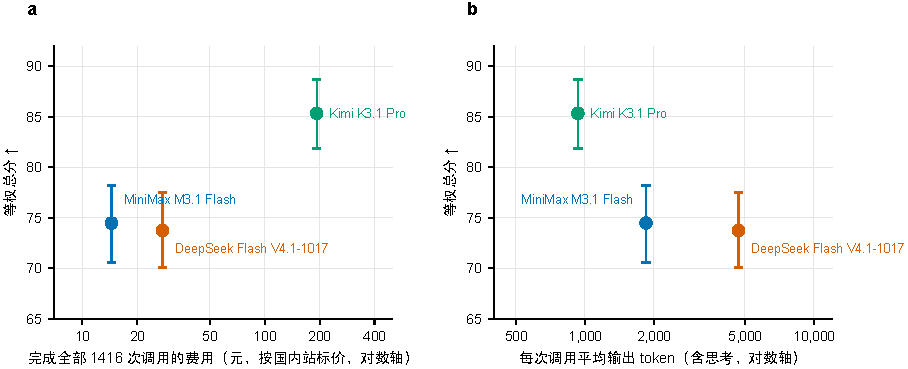
\includegraphics[width=\linewidth]{figures/fig5_cost.pdf}
  \caption{\textbf{得分与费用、输出长度的关系。}纵轴为等权总分及其 95\% 区间。(a) 横轴为完成全部评测的费用（国内站标价）；(b) 横轴为每次调用的平均输出 token。\mini 与 \ds 得分相当，\mini 的费用约为后者的一半、输出长度约为其 40\%。}
  \label{fig:cost}
\end{figure}

\begin{figure}[t]
  \centering
  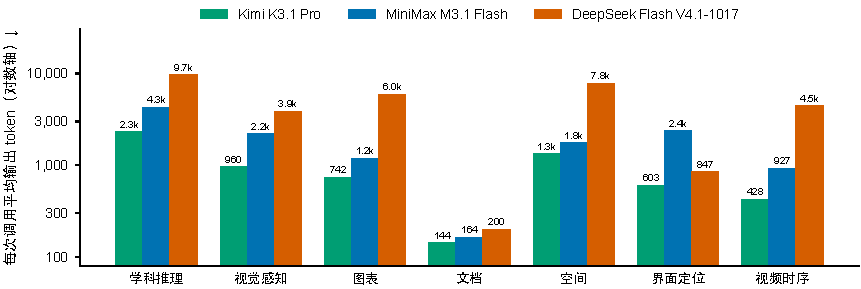
\includegraphics[width=\linewidth]{figures/fig7_tokens.pdf}
  \caption{\textbf{各项能力每次调用的平均输出 token（对数轴）。}\ds 在除界面定位外的每一项上输出都最长；文档题三个模型的输出都很短。}
  \label{fig:tokens}
\end{figure}

\section{评分规则的鲁棒性}
\label{sec:robust}

规则评分的风险在于：格式稍有偏差的正确回答可能被判为错。我们检查了全部 4,248 条回答（3 个模型 × 1416 次）：没有一条读不出最终答案，没有一条因输出上限被截断，也没有生成超时；界面定位的 600 条回答全部使用了要求的 0--1000 相对坐标。数值题的回答常带单位或量级词（如 “51 million”），评分时按数值比较，因此不会因单位写法被误判。这说明在本文的提示词下，三个模型都能稳定地遵守作答格式，分数差异来自答案本身。

规则评分仍可能把写法不同的正确答案判错。我们逐条复核了 CharXiv 推理题的全部 0 分回答，发现两道题存在误判，三个模型各有 5 条正确回答被判为 0 分。一道题的标准答案是带符号的表达式“$\bar{T}_\lambda = 2$”，回答只写出数值“2”或用 LaTeX 写出同一表达式；另一道题的标准答案是“The first graph”，回答只写“first”。另有一道题的标准答案为图中的缩写“Pass.”，回答写作全称“Passive”，是否正确无法确定，未计入。由于三个模型的误判条数相同，修正后三者的图表得分各增加 2.5 分、总分各增加 0.4 分，两两差值与排名都不变；本文报告的是修正前的分数。

\section{结论}

我们提出了 mmBench，一个以能力画像为先、同时给出可量化排名的多模态评测基准。它把多模态能力划分为 7 项，每项只考一种技能、只用一类答题形式，并用规则评分、多次采样与配对 bootstrap 给出带区间的画像与排名。对三个国产模型的评测表明：\kimi 在各项上均处于领先，但代价是 7 到 13 倍的费用；\mini 与 \ds 总分无法区分，却在界面定位与空间上方向相反，这类差异只有在能力画像中才能看到。把这些差异与厂商公开的技术要点对照，\kimi 的坐标监督与 \mini 的电脑操作方向都与它们在界面定位上相对 \ds 的领先一致，\ds 在高分辨率界面上的短板则与其接口的图片缩放上限相符；但这些都是观测上的一致，确认因果仍需对照实验。后续工作包括：加入更多模型以检验能力之间是否确实独立，补充第二个视频时序来源与更高难度的题目，并加入人类基线。

\section*{局限性}

\begin{itemize}[leftmargin=1.6em]
  \item \lead{能力的独立性是设计属性，尚未经数据验证。}判断两项能力是否真正独立，需要在大量模型上计算得分相关性；本文只评测了 3 个模型，无法完成这一检验。
  \item \lead{难度档按来源划分，未经校准。}L1--L3 反映的是来源对当前模型的饱和程度，而非逐题测得的难度；题库中没有 L4 档。
  \item \lead{部分来源接近天花板或地板。}三个模型在 DocVQA 上都在 93.8 至 94.4 分，区分度有限；\ds 在 ScreenSpot-Pro 上只有 8.3 分，接近地板。
  \item \lead{视频只有一个来源，且以抽帧代替原生视频。}视频时序全部来自 TimeBlind；统一的 16 帧协议保证了可比性，但不测厂商原生的视频输入能力。
  \item \lead{随机水平在各项之间不同。}随机猜测得分从 0 到 50 不等，等权总分把这些不同起点的分数直接平均。
  \item \lead{归因是观测上的一致，而非因果。}三个模型在数据、规模与训练方法上同时不同，本文既没有消融实验，也没有评测各自的上一版本；“一致”只说明观测与厂商声称不矛盾。厂商的视觉推理成绩多在带工具的条件下取得，而本文不提供工具。
  \item \lead{没有人类基线，评测对象有限。}本文只评测了 3 个模型在 2026 年 10 月底的接口版本；接口模型会持续更新，结果只代表评测时的状态。
  \item \lead{费用存在不确定性。}费用按公开标价与计费 token 计算，不含可能的缓存写入等费用，也不代表订阅套餐的实际支出。
\end{itemize}

\bibliographystyle{unsrtnat}
\bibliography{refs}

\appendix
\section{各来源得分}
\label{app:source}

\begin{table}[H]
  \centering
  \caption{\textbf{各来源子集上的得分（$\uparrow$）。}每行最高分加粗，次高分加下划线；“随机”为随机猜测的期望得分。各来源只是抽样子集，得分不等于该评测集的完整成绩，也不能与其官方榜单直接比较。}
  \label{tab:source}
  \small
  \begin{adjustbox}{max width=\linewidth}\begin{tabular}{llcrrrrr}
\toprule
能力 & 来源 & 难度 & 题数 & 随机 & Kimi K3.1 Pro & MiniMax M3.1 Flash & DeepSeek Flash V4.1-1017 \\
\midrule
学科推理 & MMMU-Pro & L1/L2/L3 & 50 & 12.9 & \textbf{82.0} & \underline{75.0} & 73.5 \\
视觉感知 & BLINK & L2 & 54 & 34.3 & \textbf{89.8} & 73.6 & \underline{79.2} \\
图表 & ChartQA & L1 & 15 & 0.0 & \textbf{86.7} & \textbf{86.7} & \textbf{86.7} \\
图表 & CharXiv & L3 & 35 & 0.0 & \textbf{71.4} & \underline{67.9} & 66.4 \\
文档 & DocVQA & L1 & 30 & 0.0 & \textbf{94.4} & 93.8 & \underline{94.3} \\
文档 & OCRBench-KIE & L2 & 20 & 0.0 & \textbf{79.9} & 71.3 & \underline{76.2} \\
空间 & CV-Bench-3D & L1 & 14 & 50.0 & \textbf{98.2} & \underline{92.9} & \textbf{98.2} \\
空间 & BLINK 空间子任务 & L2 & 16 & 50.0 & \textbf{87.5} & 71.9 & \underline{79.7} \\
空间 & MindCube & L3 & 20 & 30.0 & \textbf{95.0} & 56.2 & \underline{75.0} \\
界面定位 & ScreenSpot-v2 & L1 & 20 & 3.3 & \textbf{100.0} & \underline{91.2} & 78.8 \\
界面定位 & ScreenSpot-Pro & L3 & 30 & 0.0 & \textbf{60.8} & \underline{35.0} & 8.3 \\
视频时序 & TimeBlind & L3 & 50 & 50.0 & \textbf{91.0} & \underline{85.5} & 84.5 \\
\bottomrule
\end{tabular}
\end{adjustbox}
\end{table}

\begin{table}[H]
  \centering
  \caption{\textbf{逐项两两比较的逐题胜、平、负题数与得分差。}以题目的 4 次平均分比较；$^{*}$ 表示配对 bootstrap 的 95\% 区间不含 0。}
  \label{tab:wtl}
  \small
  \begin{adjustbox}{max width=\linewidth}\begin{tabular}{l*{3}{rr}}
\toprule
 & \multicolumn{2}{c}{Kimi − MiniMax} & \multicolumn{2}{c}{Kimi − DeepSeek} & \multicolumn{2}{c}{MiniMax − DeepSeek} \\
\cmidrule(lr){2-3}\cmidrule(lr){4-5}\cmidrule(lr){6-7}
能力 & 胜 / 平 / 负 & 分差 & 胜 / 平 / 负 & 分差 & 胜 / 平 / 负 & 分差 \\
\midrule
学科推理 & 9 / 39 / 2 & +7.0$^{*}$ & 11 / 39 / 0 & +8.5$^{*}$ & 4 / 42 / 4 & +1.5 \\
视觉感知 & 18 / 34 / 2 & +16.2$^{*}$ & 8 / 45 / 1 & +10.6$^{*}$ & 9 / 31 / 14 & -5.6 \\
图表 & 5 / 43 / 2 & +2.5 & 5 / 42 / 3 & +3.5 & 6 / 39 / 5 & +1.0 \\
文档 & 9 / 41 / 0 & +3.8$^{*}$ & 4 / 45 / 1 & +1.5 & 2 / 41 / 7 & -2.3$^{*}$ \\
空间 & 20 / 29 / 1 & +22.0$^{*}$ & 14 / 34 / 2 & +10.5$^{*}$ & 6 / 29 / 15 & -11.5$^{*}$ \\
界面定位 & 21 / 23 / 6 & +19.0$^{*}$ & 30 / 20 / 0 & +40.0$^{*}$ & 24 / 23 / 3 & +21.0$^{*}$ \\
视频时序 & 8 / 40 / 2 & +5.5 & 7 / 42 / 1 & +6.5$^{*}$ & 4 / 42 / 4 & +1.0 \\
\midrule
全部 & 90 / 249 / 15 & +10.9$^{*}$ & 79 / 267 / 8 & +11.6$^{*}$ & 55 / 247 / 52 & +0.7 \\
\bottomrule
\end{tabular}
\end{adjustbox}
\end{table}

\begin{table}[H]
  \centering
  \caption{\textbf{各项能力每次调用的平均输入与输出 token。}token 数为各厂商的计费用量，跨厂商不可直接比较。}
  \label{tab:tokcap}
  \small
  \begin{adjustbox}{max width=\linewidth}\begin{tabular}{l*{3}{rr}}
\toprule
 & \multicolumn{2}{c}{Kimi K3.1 Pro} & \multicolumn{2}{c}{MiniMax M3.1 Flash} & \multicolumn{2}{c}{DeepSeek Flash V4.1-1017} \\
\cmidrule(lr){2-3}\cmidrule(lr){4-5}\cmidrule(lr){6-7}
能力 & 输入 & 输出 & 输入 & 输出 & 输入 & 输出 \\
\midrule
学科推理 & 1,231 & 2,318 & 1,236 & 4,267 & 615 & 9,700 \\
视觉感知 & 3,172 & 960 & 3,148 & 2,211 & 1,349 & 3,888 \\
图表 & 929 & 742 & 1,040 & 1,191 & 464 & 5,964 \\
文档 & 3,729 & 144 & 2,856 & 164 & 844 & 200 \\
空间 & 1,226 & 1,328 & 1,329 & 1,762 & 686 & 7,810 \\
界面定位 & 6,283 & 603 & 2,962 & 2,377 & 1,048 & 847 \\
视频时序 & 25,464 & 428 & 25,459 & 927 & 10,862 & 4,451 \\
\bottomrule
\end{tabular}
\end{adjustbox}
\end{table}

\section{提示词}
\label{app:prompts}

每道题的提示词由题目、选项（若有）与作答格式说明三部分组成，以空行分隔；图片或视频帧位于文字之前。作答格式说明按题型取以下四种之一（原文为英文）：

{\raggedright
\begin{itemize}[leftmargin=1.6em]
  \item 选择题：\texttt{Answer with the letter of the correct option. End your reply with a line of the form "Answer: X".}
  \item 是非题：\texttt{Answer yes or no. End your reply with a line of the form "Answer: yes" or "Answer: no".}
  \item 短答案：\texttt{Answer with a single word, number or short phrase. End your reply with a line of the form "Answer: <your answer>".}
  \item 坐标：\texttt{Give the point as relative coordinates: x from the left edge and y from the top edge of the image, each an integer from 0 to 1000. End your reply with a line of the form "Answer: (x, y)".}
\end{itemize}
\par}

选择题的选项以 “A. …”“B. …” 的形式逐行列出；选项已写在题目中或图片中的题不再重复列出。视频题在帧之前加一句：\texttt{The following 16 images are frames sampled uniformly from a video, in order.}

\section{复现}
\label{app:repro}

代码、题号清单与本文的全部图表脚本见 \url{https://github.com/BAI-AI-Lab/mmBench}。题目、图片与视频帧不随仓库发布，需按以下命令从原始来源重新构建（在来源数据集未变动的前提下，固定种子保证得到同一套题；仓库的每周 CI 会检查各来源是否仍可访问并能抽满题数）：

\begin{small}
\begin{verbatim}
bash install.sh                    # Python 环境
bin/mmb build                      # 按来源与 seed = 0 构建题库
export MODEL=... OPENAI_BASE_URL=... OPENAI_API_KEY=...
REASONING_EFFORT=max bin/mmb run   # 每题 4 次，结束后生成单模型报告
bin/mmb report runs/A/mm-full runs/B/mm-full --out reports/A_vs_B
\end{verbatim}
\end{small}

运行中断后重跑同一条命令只补未完成的题；同一运行目录同一时间只允许一个进程，避免重复请求。本文的分析数字、表格与图由仓库 \texttt{paper} 目录下的三个脚本从各运行的日志生成：\texttt{analysis.py} 计算全部统计量，\texttt{make\_tables.py} 生成表格，\texttt{make\_figures.py} 绘图。


\vspace{2em}\begin{flushright}由 Albert Huang 创建于 2026-10-31\end{flushright}

\end{document}
